\documentclass[a4paper,14pt]{extreport}
\usepackage[left=1.5cm,right=1.5cm,
    top=1.5cm,bottom=1.5cm,bindingoffset=0cm]{geometry}
\usepackage{scrextend}
\usepackage[T1,T2A]{fontenc}
\usepackage[utf8]{inputenc}
\usepackage[english,russian,ukrainian]{babel}
\usepackage{tabularx}
\usepackage{amssymb}
\usepackage{color}
\usepackage{amsmath}
\usepackage{mathrsfs}
\usepackage{listings}
\usepackage{graphicx}
\graphicspath{ {./images/} }
\usepackage{lipsum}
\usepackage{xcolor}
\usepackage{hyperref}
\usepackage{tcolorbox}
\usepackage{tikz}
\usepackage[framemethod=TikZ]{mdframed}
\usepackage{wrapfig,boxedminipage,lipsum}
\mdfdefinestyle{MyFrame}{%
linecolor=blue,outerlinewidth=2pt,roundcorner=20pt,innertopmargin=\baselineskip,innerbottommargin=\baselineskip,innerrightmargin=20pt,innerleftmargin=20pt,backgroundcolor=gray!50!white}
 \usepackage{csvsimple}
 \usepackage{supertabular}
\usepackage{pdflscape}
\usepackage{fancyvrb}
%\usepackage{comment}
\definecolor{ggreen}{rgb}{0.4,1,0}
\definecolor{amber}{rgb}{1.0, 0.75, 0.0}
\definecolor{babyblue}{rgb}{0.54, 0.81, 0.94}
\definecolor{arylideyellow}{rgb}{0.91, 0.84, 0.42}
\usepackage{array,tabularx}
\usepackage{colortbl}

\usepackage{varwidth}
\tcbuselibrary{skins}
\usepackage{fancybox}

\usetikzlibrary{calc}
\makeatletter
\newlength{\mylength}
\xdef\CircleFactor{1.1}
\setlength\mylength{\dimexpr\f@size pt}
\newsavebox{\mybox}
\newcommand*\circled[2][draw=blue]{\savebox\mybox{\vbox{\vphantom{WL1/}#1}}\setlength\mylength{\dimexpr\CircleFactor\dimexpr\ht\mybox+\dp\mybox\relax\relax}\tikzset{mystyle/.style={circle,#1,minimum height={\mylength}}}
\tikz[baseline=(char.base)]
\node[mystyle] (char) {#2};}
\makeatother

\usepackage{float}
\usepackage{wrapfig}
\usepackage{framed}


\begin{document}
\pagecolor{white}


\begin{center}
Variant №4\\
\vspace{0.5cm}
Bohdan Lyshchenko DP-82
\end{center}

\begin{center}
Які принципи покладені у класифікацію механізмів поляризації?
\end{center}
\vspace{1cm}



If we are talking about the \underline{physical} mechanisms of elastic polarization, then schematically this can be shown in Fig.\ref{ris1}

\begin{figure}[h]
\center{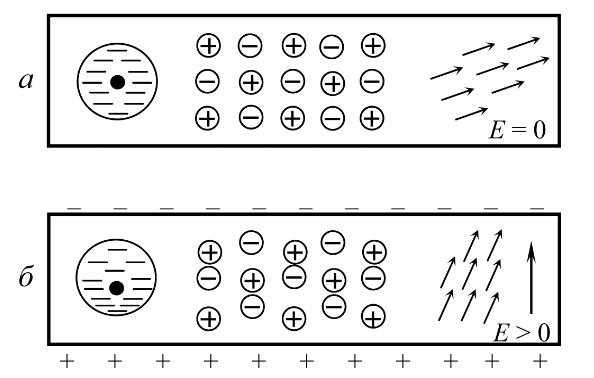
\includegraphics[width=0.5\linewidth]{1.png}}
\caption{Physical mechanisms of elastic polarization (a, b - three mechanisms of elastic polarization - fragments of the dielectric without the application of an electric field E and in the case of its inclusion).}
\label{ris1}
\end{figure}

But if you turn off the applied external field, all of the considered mechanisms provide an elastic return of the system of charges to an equilibrium unperturbed state (Fig.\ref{ris1}, a). The electrons will occupy a symmetrical position relative to the nuclei due to the Coulomb force of attraction to the nucleus; the cations and anions will return to their stable (equilibrium) position in the nodes of the crystal lattice under the action of the repulsive force of the electron shells of the ions. \\

If an electric field is applied (Fig.\ref{ris1}, b), then in each atom, molecule, and ion the electronic orbitals are deformed and shifted relative to the nuclei, causing the center of the negative charge to shift relative to the positively charged nucleus. Thus, in each structural element there is an elementary polarizability p = qx> 0. This is the mechanism of electronic elastic polarization.

In an electric field applied to a dielectric, bound electric charges shift relative to each other, causing the dielectric to become polarized (that is, polarization is the separation of charges, whereas electrical conductivity is the transfer of charges). The external electric field induces elementary electric moments p = qx in the dielectric particles.
In the formation of such a field-induced electric moment can take part: \\

- electrons shifting from equilibrium states in atoms relative to positively charged nuclei; \\

- ions, deviating from the equilibrium state in the crystal lattice; \

- dipoles, polar molecules or radicals that change their orientation under the action of the field. \\

In addition to elastic polarization, electrons, ions, and dipoles (or macrodipoles) can also participate in thermal and migration polarization mechanisms.














\end{document}
